%************************************************
\chapter{Curating a set of orthologous mammalian gene trees}
\label{ch_orthologs}
\acresetall
%************************************************

\section{Introduction}

This chapter considers the identification of groups of orthologous
genes in vertebrates and mammals. I begin with a discussion of the
detection of orthologs within groups of vertebrate and other
eukaryotic genomes, focusing on the tree-based approach to ortholog
and paralog identification as used by the Optic, \cmp, and Treefam
databases. In preparation for the sitewise analysis of mammalian
orthologs to be presented in the subsequent two chapters, I construct
a simple method for isolating \subtr{}s with largely orthologous
characteristics from the set of \cmp gene trees and analyze the
taxonomic distribution of gene duplication and loss within those
\acp{lot}, demonstrating how strongly the history of genome
duplications has affected the structure of orthologous and paralogous
relationships between and within vertebrate and invertebrate
genomes. The set of gene trees resulting from a simple tree-splitting
process based on taxonomic coverage is selected for use in the
subsequent sitewise analysis.

\section{Methods for ortholog identification}

Central to any evolutionary sequence analysis is the assumption that
the sequences being analyzed, or some parts therein, share a common
evolutionary origin. Thus, the first step in any such analysis is the
collection of homologous sequence data. Starting with a source
sequence, homologs are usually identified by searching a sequence
database for sequences with a minimum overall similarity according to
some evolutionary model. In some cases, such as when sequences are
highly divergent or subject to domain shuffling or horizontal gene
transfer, a more localized or more specialized measure of similarity
may be desirable \citep{Koonin2001,Sjolander2011}, but within closely
related groups of organisms such as vertebrates and mammals, the
process of gene duplication and divergence dominates patterns of
relatedness between protein sequences \citep{Ohno1970}, making overall
sequence similarity a useful method by which to identify homologous
sequences in the organisms of interest.

Heuristic algorithms have been developed for performing quick and
sensitive sequence homology searches within databases of protein and
nucleic acid sequences \citep{Altschul1997,Eddy2009}. The power of
these methods is high enough that homology within vertebrates, even
for fast-evolving genes, can be readily detected. However, the
prevalence of historical and ongoing gene duplication and loss in
vertebrates complicates the problem, as orthologous genes (e.g.,
homologs between species, sharing a common ancestral population and
related through a speciation event) and paralogous genes (e.g.,
homologs within a single species, sharing a common ancestral genomic
sequence and related through a duplication event) are important, yet
difficult, to distinguish from one another \citep{Jun2009}. In other
words, sets of genes that may be confidently identified as sharing
homology may still contain paralogy and orthology relationships that
are more difficult to resolve. Since the evolutionary trajectories of
paralogous versus orthologous genes are expected to be quite distinct
\citep{Lynch2000}, the correct identification of orthologous versus
paralogous relationships in vertebrates is critical for any detailed
molecular evolutionary analysis.

Methods for distinguishing orthologous from paralogous relationships
within vertebrate genomes have been in development for over a decade
\citep{Remm2001,Yuan1998}, but the amount of overlap between
vertebrate orthologous groups identified by different methods has
historically been disappointingly small \citep{Jun2009,Chen2007},
suggesting that the problem of orthology inference is far from
resolved. Still, one might expect the accuracy and power of orthology
inference methods to improve with time, given the steady increase in
available computing power and the sequencing of many complete
vertebrate genomes over the past decade. Indeed, the growing number of
available sequenced genomes, greater available computational power,
and improved understanding of patterns of gene duplication and loss
have led to the growing popularity of phylogeny-based approaches,
which were once considered computationally impractical and too
difficult to automate \citep{Remm2001}. In general, the phylogenetic
approach involves estimating a phylogenetic tree from an entire
cluster of homologous genes and inferring duplication events based on
the discordance between the gene tree and the species tree. Several
variants of this approach have been developed and applied to gene tree
reconstruction in insects, fungi and vertebrates
\citep{Muller2010a,Cepas2007,Datta2009,Vilella2009,Ruan2008,Hahn2007a},
and validation against manually-curated gene trees has shown these
phylogeny-based methods to be more sensitive and accurate than
pairwise or graph-based methods \citep{Datta2009}.

One particular phylogeny-based approach, which uses a known species
tree to guide the resolution of orthologs and paralogs within a gene
tree in a Bayesian framework, has been implemented in a software
package called TreeBeST and used extensively to infer genome-wide
vertebrate and eukaryotic gene trees for the Optic, TreeFam and \cmp
databases \citep{Heger2008,Ruan2008,Vilella2009}.

I describe in this chapter an initial analysis of the gene trees
within \cmp which I undertook in preparation for the sitewise
evolutionary analysis presented in Chapters \ref{ch_mammals1} and
\ref{ch_mammals2}. The major goals of this analysis were to better
understand the distribution of orthologous genes within vertebrate
genomes, identify which taxonomic constraints would best define
largely-orthologous groups of mammalian genes, and evaluate whether
\lcv genomes, which are unique to the Compara database of
orthologs, showed high enough annotation quality and consistency to be
included in the mammalian evolutionary analysis. Throughout the
chapter, attention will be paid to those aspects of the gene tree
identification pipeline which may contribute to errors in the
downstream evolutionary analysis.

\section{Low-coverage genomes in the Ensembl database}

A major feature that distinguishes \cmp from the Treefam and Optic
databases is the inclusion in \cmp of several mammalian genomes which
have been sequenced to low coverage as a part of the \ac{mgp}. The
inclusion of these additional genomes was a major reason why I
performed the analysis described in the following chapters using
Ensembl as a source of gene trees and alignments, representing a major
advantage over otherwise similar orthology databases due to the
greater species sampling density. With respect to the actual
sequencing of the \lcv mammalian genomes, the motivation and goals of
the \ac{mgp} itself will be outlined in the next chapter. For the
purpose of the present discussion, I will outline the way \lcv genomes
are handled within the Ensembl annotation pipeline, as certain
features of the \lcv genomes cause characteristic anomalies in the
orthology analyses, as will be shown in the ensuing analysis.

The prevalence of missing sequence data and fragmented contigs in \lcv
genomes presented a unique set of problems for the generation of
transcript annotations in \ens. In recognition of these differences,
the procedure used by \cmp to annotate genomes assembled from \lcv
data is distinct from the usual gene-building pipeline
\citep{Hubbard2007}. Briefly, a whole-genome alignment is produced
between the human genome and each \lcv target genome, and gene models
are projected from human to the target genome. Small frame-disrupting
insertions or deletions within orthologous exons are corrected, and
missing or incomplete exons are padded with Ns in order to produce a
transcript with a length equal to that of the human reference
transcript. The inclusion of these error-correcting features allows
for a set of intact, if not complete, coding transcripts to be
generated for \lcv genomes, leveraging the high level of sequence
similarity between human and other \euth mammals to project genes
and transcripts from the high-quality human genome to the unannotated,
highly fragmented \lcv genome assemblies. Still, in many cases the
\ens pipeline could not map complete genes or transcripts from human
to the target genome, causing difficulty in identifying
duplications. On one hand, the lack of completely assembled
chromosomes meant that segmental duplications in \lcv genomes were
often unresolved or unidentifiable, making it difficult or impossible
to confidently identify recently duplicated genes. On the other hand,
the shorter length of assembled fragments caused genes to occasionally
be split between two sequence fragments; the \ens pipeline currently
annotates such genes as two separate shortened gene fragments,
resulting in an excess of shortened apparent paralogs in resulting
gene trees (see Section \ref{sub_removing_paralogs} for more detail on
this artifact).

The \cmp gene family pipeline, which I describe in more detail below,
uses the set of annotated transcripts from each species as its input
\citep{Vilella2009}, so the quality of gene annotation from each
source genome has a direct impact on the overall quality and accuracy
of the resulting gene trees. Although the reliance on genome-wide
alignments to, and gene annotations from, a reference genome could be
criticised for potentially causing a bias towards the genomic
properties of the reference, this approach is a reasonable workaround
in the absence of higher-coverage sequence data or a painstakingly
curated assembly. Furthermore, the gene model error-correcting
features of the Ensembl pipeline are especially beneficial, making
more complicated methods for correcting errors from \lcv genomes such
as those described by \citep{Hubisz2011} seem less necessary.

\section{The Ensembl Compara gene tree pipeline}
\label{section_compara_pipeline}

All genomic data and gene trees used for this analysis were sourced
from version 63 of the Ensembl Compara database
\citep{Vilella2009,Flicek2011}. Although a complete description of the
design, implementation, and validation of the pipeline behind the
Ensembl database would be beyond the scope of this chapter, I will
briefly outline the major aspects of the approach used by the Compara
pipeline, focusing on a few details which are relevant to the current
analysis and ensuing discussion.

The Compara pipeline begins with a set of protein-coding transcripts
collected from each individual species' annotation database. This step
is not exactly straightforward, however, as the prevalence of
alternative splicing in \euth mammals makes it common for a single
gene to harbor many different transcript structures.

In terms of biology and evolution, alternative splicing is a very
interesting phenomenon. Tightly linked to the evolutionary innovation
of regulatory control and tissue-specific gene expression, the
existence of multiple transcripts per gene is one of the likely
substrates of biological and developmental complexity within
vertebrates and mammals as compared to single-celled eukaryotes, which
show less developmental complexity but largely similar numbers of
genes \citep{Csuros2011}. Further evidence of the unique evolutionary
characteristics of alternatively-spliced exons comes from molecular
evolutionary studies which have shown such exons to show, on average,
higher levels of evolutionary constraint, possibly owing to the
importance of exonic splice enhancers in modulating the inclusion or
exclusion of their associated exons \citep{Parmley2006}.

In terms of organizing biological data, however, pervasive alternative
splicing is somewhat burdensome. Roughly 34\% of human genes contain
at least two, and up to several dozen, transcripts per gene
\citep{Mironov1999}, showing tissue-specific and species-specific
expression patterns, different levels of overall transcription, and
sometimes comprising mutually exclusive exons. Within the context of
the Compara database, the first problem in maintaining consistency
across many source genome sequences is the fact that primary data on
alternative transcript structures (e.g., data from expressed sequence
tags, RNA-seq, or proteomics experiments) are largely absent from most
organisms with sequenced genomes. Furthermore, the task of
incorporating multiple transcripts per gene into an evolutionary
framework is non-trivial, and leaves many unresolved questions open to
debate: should all transcripts be treated as independent evolutionary
entities, or should some form of meta-transcript be produced,
comprising all possible transcripts for a given gene? Should
expression levels and tissue-specificity be taken into account (as
both factors have been correlated with evolutionary rate,
e.g. \citep{Koonin2006a,Zhu2008})? And what is the expected
evolutionary impact of the loss, gain, or modulation of the prevalence
or tissue-specificity of a given exon or transcript in one lineage?
Even a fairly shallow consideration of the topic quickly reveals
layers of complexity that would quickly hinder many large-scale
evolutionary analyses, such as the definition of orthologous groups,
whose main goals are to understand the evolutionary relationships of
gene families within some set of species' genomes.

As a result of these difficulties, the current design of the Compara
pipeline only incorporates one 'canonical' transcript per gene into
the evolutionary analysis and the resulting inferred gene trees. This
reflects a conscious decision to sacrifice some biological fidelity
for reduced design complexity and computational load, as the inclusion
of multiple transcripts would inevitably require some amount of
additional processing and/or calculation. Unfortunately, this only
somewhat alleviates the problem, shifting the burden from ``how to
deal with multiple transcripts in a comparative setting'' to ``how to
choose the best representative transcript for each gene.'' In the case
of a gene with many transcripts of varying sizes containing many
non-overlapping exons, the negative consequences of choosing a
non-optimal transcript are clear: too short of a transcript could
exclude important sequence information from the dataset, while
transcripts with spurious exons (resulting from misannotation or
erroneous experimental evidence for a transcript) could introduce
potentially large amounts of non-orthologous, nonfunctional, or
nonconserved sequence into the evolutionary analysis.

Fortunately, the consensus coding sequence (CCDS) project was
initiated in 2005 to ``identify a core set of human and mouse protein
coding regions that are consistently annotated and of high quality''
\citep{Pruitt2009}. Although the transcripts that satisfy these two
criteria will not necessarily be the same as those which meet the
desired definition of ``the best representative transcript for use in
an evolutionary study,'' the confidence that one can have in the
quality and consistency of CCDS transcripts helps to reduce the
prevalence of potentially damaging errors in the Compara pipeline.
Thus, in the current release (version 63), the ``representative''
transcript used for the Compara pipeline is chosen on the basis of (a)
existence within the CCDS set of transcripts and (b) the total length
of the transcript's coding sequence. The combination of these two
factors can be expected to identify a reasonably representative
transcript, at least for the human and mouse genomes. The situation
will be similar for genomes whose Ensembl annotation is derived
largely from synteny and orthology to human and mouse annotated genes,
but two classes of genomes---those resulting from low-coverage
sequencing and those from more distant species whose annotations are
derived from largely independent data sources---will still suffer from
some amount error in the form of poor transcript choice. The OPTIC
database, which contains orthologous groups identified within a wide
range of animal and fungal clades, uses the transcript with the
maximum length as the canonical transcript \citep{Heger2008}.

Once the set of canonical transcripts is chosen, an all-against-all
protein BLAST search is performed using the Washington University
variant of BLAST and genes are clustered into homologous groups using
\hclust, an implementation of a hierarchical clustering algorithm for
sparse graphs. Sequences are aligned using MCoffee, a meta-aligner
algorithm which combines the results from different aligners into one
alignment using a maximum-consistency criterion
\citep{Wallace2006}. The aligners used for the M-Coffee alignment
include MAFFT \citep{Katoh2005}, MUSCLE \citep{Edgar2004}, KAlign
\citep{Lassmann2009}, and T-Coffee \citep{Notredame2000}. Finally, the
aligned sequences are input to TreeBeST, which infers a gene tree
(including gene duplication and loss events) given a set of aligned
sequences and a known species tree \citep{Ruan2008}. The type of the
homology relationship between each pair of genes (e.g., one-to-one
ortholog, one-to-many ortholog, within-species paralog) is determined
using a simple set of rules based on the structure of the inferred
gene tree and the annotation of ancestral nodes where a duplication
event has likely occurred.

The Compara pipeline has been a part of the Ensembl ecosystem since
its first introduction to Ensembl in release 42
\citep{Birney2006}. Remarkably, aside from slight tweaks to the
protein clustering method and some changes in the exact aligners used,
the pipeline has changed little from its original published form
\citep{Vilella2009}. In part, this lack of change reflects the ease
with which sets of vertebrate orthologs can be identified using the
existing methodology, lying in contrast to the equivalent task in sets
of insect or fungal genomes where divergence levels between extant
species with sequenced genomes are much larger \citep{Siepel2005} and
the shape of the underlying species tree may be uncertain and/or
unknown \citep{MacKenzie2008a}, making the development of specialized
methods or extensive manual annotation necessary
\citep{Kellis2004,Rasmussen2007}. This is equivalent to saying that
Ensembl's pipeline, while not perfect in its orthology predictions or
tree inferences (as indicated in a series of back-and-forth papers
between Milinkovitch et al. \citeyearpar{Milinkovitch2010} and Villela
et al. \citeyearpar{Vilella2011}), has proved sufficiently accurate
enough that an extensive reworking of the system has not yet been
deemed necessary. However, it is worth noting that the recent
development of a new Bayesian method for gene tree reconciliation,
based on a generative model of gene family evolution as a birth-death
process and incorporating species-specific and gene-specific rate
variation, showed good performance in resolving fungal and
invertebrate gene trees, and could easily be adapted to the vertebrate
genomes in the Compara database . Additional validation of the overall
approach taken by Compara comes in the form of Treefam and Optic
\citep{Ruan2008}, databases of animal and fungal gene trees which
applied a similar set of tools to infer gene trees from a more diverse
set of genomes, producing qualitatively similar results
\citep{Vilella2009}.

\section{Quantifying paralogous relationships within Ensembl gene trees}
\label{section_quantifying_paralogous}

The first task in preparing the \cmp data for subsequent sitewise
analysis was to identify and extract a set of gene trees or gene
\subtr{}s comprising largely of orthologous relationships within
mammals (i.e. \acp{lot}), avoiding as much as possible the inclusion
of paralogous relationships. It was necessary to postprocess the \cmp
gene trees in order to achieve this goal, because many of the \cmp
trees contained multiple sets of complete \mammln orthologous trees
linked by ancient gene duplication events, while I wished to study the
evolution of each \mammln \ac{lot} in isolation. In other words, the
Compara gene trees could be charcterized as being over-clustered with
respect to the core set of \mammln orthologous trees. This
over-clustering was not necessarily inaccurate with respect to the
evolutionary history of vertebrate genes, but it was not a desirable
feature for my intended use of the data. This section is concerned
with identifying and quantifying the level of such over-clustering
within the Compara database.

I first collected the set of 18,607 \cmp gene trees and analyzed their
overall size and the number of human genes contained within each
tree. The results of this analysis are presented in Table
\ref{ensembl_root_table} and Figure \ref{ensembl_roots_hist}; a
complete description of these data will follow in Section
\ref{section_root_compara_trees}, but the aspects relevant to
characterizing the amount of paralogy contained within these trees
will be discussed here.

The first row of Table \ref{ensembl_root_table} shows various summary
statistics from the full set of \cmp gene trees, with the columns
under the ``Human Content'' heading showing the fraction of all gene
trees containing zero, one, or two or more human genes. Evidence for
the existence of large numbers of paralogs within \cmp trees came from
the observation that 20\% of \cmp trees contained 2 or more human
genes. If each Compara tree contained only one set of \mammln
orthologs, then the 20\% of trees with multiple human gene copies
could only be explained by an unrealistically high rate of gene
duplication in the lineage leading towards human. Instead, a more
parsimonious explanation was that many of the Ensembl trees contained
not one group of \mammln \acp{lot}, but two or more sets of \mammln
\acp{lot} joined by one or more ancient duplication events. This
explanation was further supported by Figure \ref{ensembl_roots_hist},
which shows a histogram of total gene counts in the Ensembl root
trees. A large number of trees contained more than 48 sequences (the
number of vertebrate genomes in \ens), with clear peaks in the
histogram of trees with 2, 3, and 4 times the number of vertebrate
genomes in \ens. These patterns were highly consistent with a high
number of \cmp gene trees containing multiple \mammln \acp{lot}.

The prevalence of over-clustered \euth orthologs in the Compara
database could be explained by a combination of the \hclust algorithm
used for the hierarchical clustering step, which uses only protein
distances as its source of clustering information, and the wide range
of protein evolutionary rates in the vertebrate genome. As I mentioned
in Section \ref{section_compara_pipeline}, the Compara pipeline uses
all-by-all protein BLAST E-value scores and the \hclust algorithm to
produce sets of sequences containing minimal average within-group
E-values. No additional biological information, such as the source
species of each sequence or the overall \ac{tc} of each cluster, is
used in identifying clusters, and no attempt is made to fit clusters
to an expected model of orthologous gene evolution. On the one hand,
the lack of additional information and assumptions allows the
algorithm to remain simple and the clustering behavior to remain
consistent across different groups of genomes; on the other hand, a
number of technical (in the sense of non-biologically meaningful)
parameters and thresholds must be tuned in order to result in the
desired cluster sizes and contents. Importantly, even after these
parameters were tuned to perform well on the dataset as a whole (i.e.,
to successfully cluster a majority of vertebrate orthologs), the
reliance on protein distances alone means that fast-evolving proteins
will be more likely to be under-clustered and slow-evolving proteins
will be more likely to be over-clustered. The rate of protein
evolution varies widely within a genome, as evidenced by a study of
amino-acid substitution rates of roughly 6,000 eukaryotic orthologous
genes by Koonin et al. [\citealt{Koonin2004}], who found that the
middle 90\% of genes show a nearly fourfold variation in evolutionary
rate. Given this wide range of protein evolutionary rates, the excess
of over-clustered orthologs in the Compara database is understandable
and even somewhat expected.

Before continuing with a description of a method to identify \acp{lot}
within \cmp gene trees, I should note that my use of the phrase
``over-clustered'' refers only to over-clustering with respect to the
current goal of analyzing independent sets of orthologous genes within
\mamml{}s. Certainly these large ``over-clustered'' trees, which
represent a more distant evolutionary history than a single \mammln
orthologous group, are just as accurate with respect to the true
evolutionary history of the genes as more narrow groupings would
be. Furthermore, the inclusion of a deeper evolutionary context may
sometimes be more useful to users of the Compara database, for whom an
understanding of the overall evolutionary history of a gene may be the
topic of primary interest.

\begin{figure}
\centering
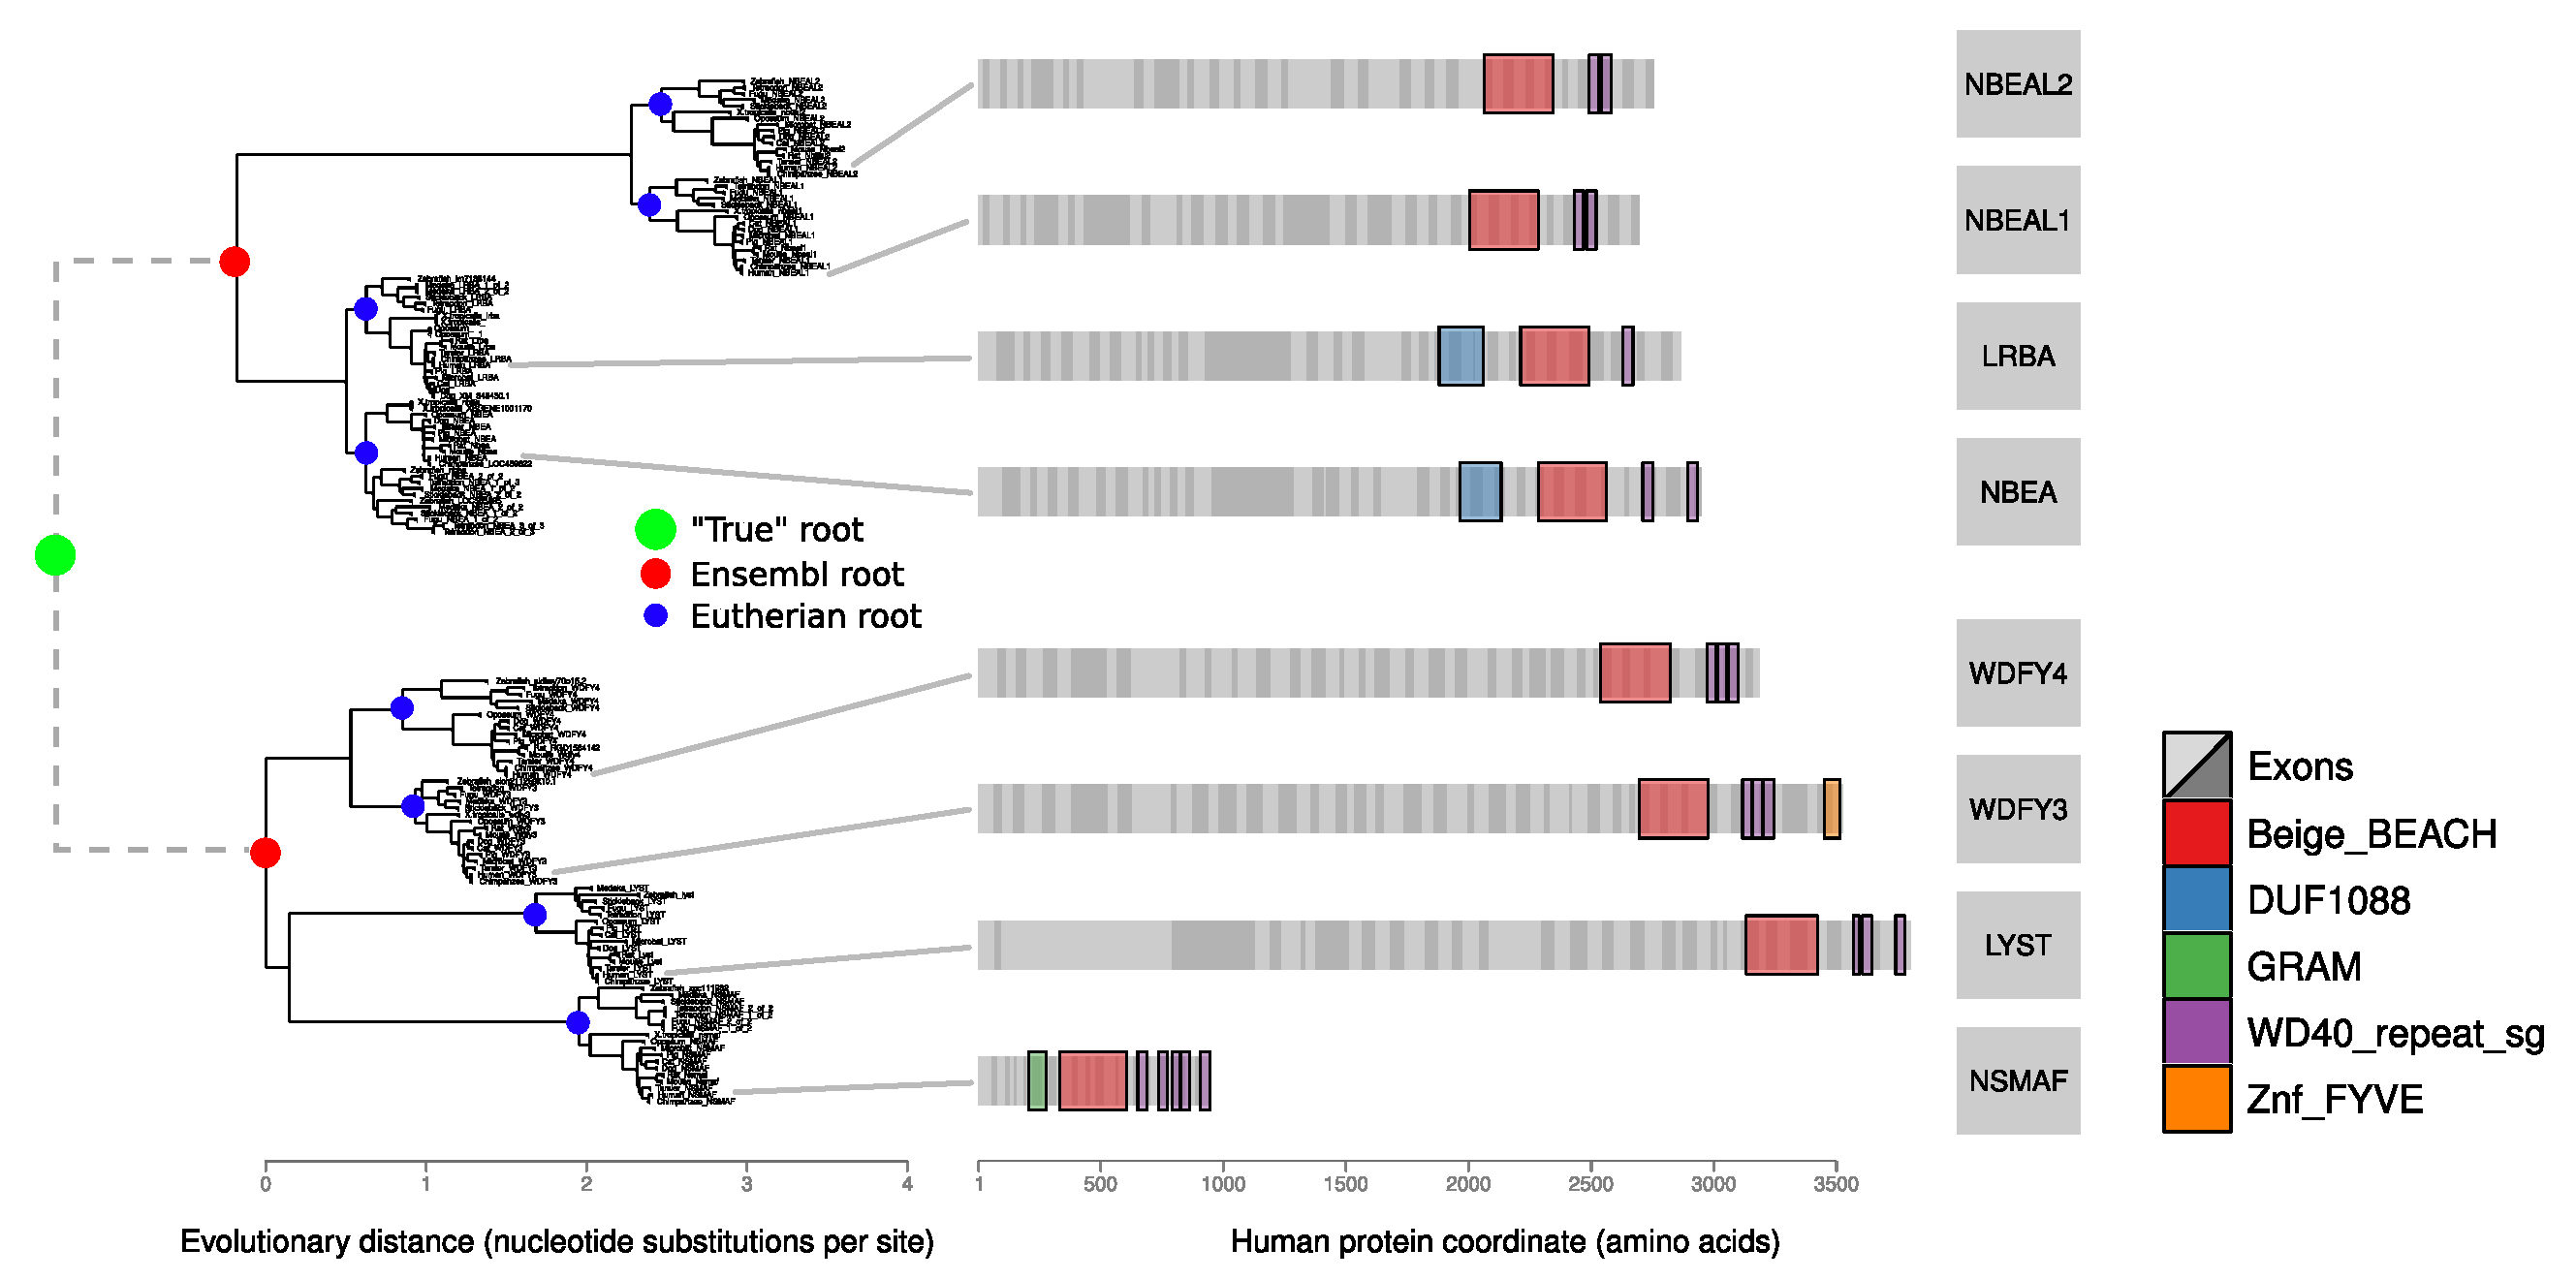
\includegraphics[scale=0.35]{Figs/nbeal2_full.pdf}
\caption{The evolutionary history of the human \gene{neurobeachin-like 2}
  gene (\gene{NBEAL2}) and its paralogs. Left, two phylogenetic trees from
  Ensembl Compara (release 60) are shown, summarizing the evolution of
  \gene{NBEAL2} and its three paralogs (top) and \gene{LYST}, a presumed distant
  paralog of \gene{NBEAL2}, and its three paralogs (bottom) in 15
  vertebrate species. The phylogeny shows that \gene{NBEAL2} is
  taxonomically conserved and distinct from its paralogs. Red dots
  highlight the root nodes of Ensembl gene trees, blue dots highlight
  the root nodes of \euth orthologous subtrees, and a dashed line
  with a green dot represents the putative paralogous relationship
  (with a hypothetical root) between the two Ensembl gene
  trees. Right, the exon and domain structure of each human gene is
  shown: exons are displayed alternating shades of gray, and Pfam
  domain annotations are colored according to their Pfam identifier.}
\label{nbeal2}
\end{figure}

As an example, take the gene \gene{NBEAL2} and its human paralogs,
whose gene trees, exon structures and domain classifications were
extracted from Ensembl v62 and summarized in Figure \ref{nbeal2}. A
recent medical sequencing project identified \gene{NBEAL2}, a gene of
previously unknown function, as the putative causative gene for gray
platelet syndrome, a predominantly recessive platelet disorder
resulting in moderate to severe bleeding \citep{Albers2011}. I
performed, with Botond Sipos, an evolutionary analysis of
\gene{NBEAL2} for the article describing the discovery, and it was
important for the purpose of this study to ensure that the
\gene{NBEAL2} gene was both well-conserved across mammals and distinct
from its paralogs. The \cmp pipeline clustered \gene{NBEAL2} with
three of its closest paralogs into one tree (and similarly clustered
four more distant \gene{NBEAL2} paralogs into a separate tree),
yielding two views which together showed both the full taxonomic
coverage of the \gene{NBEAL2} \subtr{} and the large amount of
evolutionary distance between paralogs. Had each \mammln ortholog been
displayed independently in \ens (i.e., using the blue ``\euth root''
nodes in Figure \ref{nbeal2}), it would have been more difficult for a
non-expert to make such claims regarding the evolutionary history of
\gene{NBEAL2} without further analysis. Conversely, had the \cmp
pipeline been even more inclusive in its clustering approach and
identified the hypothetical deeper root connecting these two sets of
trees (represented by the green node in Figure \ref{nbeal2}), the
connection between these eight genes would have been even more
immediately apparent.

For the purposes of this project, however, it was important to isolate
individual \mammln gene trees for further processing and sitewise
analysis. To this end, I designed a simple scheme for splitting gene
trees into non-overlapping subtrees based on flexible \ac{tc}
criteria; the remainder of this chapter presentes design and results
of this process when applied to the \cmp gene trees.

\section{Using taxonomic coverage to extract largely orthologous \mammln \subtr{}s}

Based on the observation that the clustering step of the \cmp pipeline
did not make use of any taxonomic information, I hypothesized that a
relatively simple set of rules based on \ac{tc} would be sufficient to
identify most \mammln \acp{lot}. Two well-established observations in
\mammln genomes supported the decision to use \ac{tc} in this
context. First, the existence of two rounds of whole-genome
duplication preceding the evolution of vertebrates \citep{Dehal2005}
suggested that many of the ancient duplication events contained within
Ensembl gene trees occurred before the divergence of \mamml{}s, making
it possible to cleanly separate out taxonomically complete \mammln
\subtr{}s in the majority of cases. This would not be possible if
duplication events were common and spread evenly throughout the
\mammln tree; if that were the case, many duplication events would
have occurred after the divergence of some or all of the major \mammln
groups, resulting in a larger proportion of \mammln genes with
``internal'' duplications and, thus, fewer singly orthologous trees
with high taxonomic coverage. Second, the overall low rate of gene
duplication and loss in mammals \citep{Demuth2006} (excluding, of
course, the aforementioned whole-genome duplication events which
occurred in the ancestral vertebrate genome) predicts that few \mammln
gene trees will be subject to one or more gene duplication or loss
events. In other words, most \mammln gene trees should contain
sequences from a majority of \mammln species, so the effectiveness of
using \ac{tc} to identify \mammln \subtr{}s should be largely
unaffected by continued (i.e., post whole-genome duplication) gene
duplication or loss events. The potential utility of \ac{tc} was
further bolstered by the star-like shape of the \mammln tree
\citep{BinindaEmonds2007}: a star-like trees contains more branch
length within terminal lineages than a ladder-like tree with an
equivalent total branch length, making it less likely that a gene
duplication or loss event (if such events occurred randomly throughout
the \mammln tree) would result in a significant disruption to the
\ac{tc} of the gene tree.

The \ac{tc}-based tree splitting process worked as follows. For every
internal node $N$ of each \cmp gene tree, the \ac{tc} was calculated
for several vertebrate clades. The \ac{tc} for node $N$ and clade $C$
was calculated as $TC(N,C) = species(N) / species(C) $, where
$species(N)$ is the number of unique species represented by the
sequences beneath node $N$ and $species(C)$ is the number of species
within the vertebrate clade $C$. The tree was then traversed from root
to tip, and if a given set of \acp{tcc} were satisfied by both
\subtr{}s below node $i$, then the tree was split into two \subtr{}s
at node $i$, with the new trees having root nodes placed at the two
child nodes, $i_a$ and $i_b$. The traversal continued recursively
until every node was tested against the \acp{tcc}. The smallest
\subtr{}s which satisfied the \acp{tcc} were included in the resulting
\subtr{} set. If only the entire gene tree satisfied the \acp{tcc}
then the entire tree was included; if the entire gene tree failed to
satisfy the \acp{tcc}, it was excluded altogether from the resulting
\subtr{} set.

I chose a variety of \acp{tcc} to apply to the set of \cmp trees, all
of which were run against the 18,607 gene trees within the Compara
database to generate several genome-wide \subtr sets. Table
\ref{subtree_constraints} shows the details of the various \acp{tcc}
used. The clade names (e.g., $TC(Primates)$) refer to the set of
species in the \ens database that are contained within the given
\subtr of the NCBI taxonomy; the NCBI classification of species
contained within \ens is shown in Figure \ref{ncbi_tree}, including
labels on internal nodes corresponding to the clade names given in
Table \ref{subtree_constraints}.

For the Ingroup and Outgroup categories of \acp{tcc}, a \ac{tc} value
of greater than 0.6 was required for a single taxonomic clade. This
value was not arbitrarily chosen; rather, it was important to use a
\ac{tc} value slightly above 0.5 to achieve the desired result of
identifying orthologous \subtr{}s. A value much higher would be too
restrictive: if, for example, the required \ac{tc} value were set to
1, then all subtrees containing a deletion in any species within the
clade of interest would not satisfy the \ac{tcc}. On the other hand, a
required \ac{tc} value of less than 0.5 would allow a single \ac{lot}
to be split into two \subtr{}s, with one \subtr having \ac{tc}$<0.5$,
and the other \subtr, containing the other half of the species within
the clade of interest, also having \ac{tc}$<0.5$. Thus, 0.6 was deemed
a sufficient \ac{tc} requirement for isolating \subtr{}s with
reasonably high \ac{tc} while allowing for some amount of gene
deletion.

Two additional types of \acp{tcc} were designed for use in the
MammalSubgroups and MammalSubgroupsPlusOutgoup methods. Inspired by
the alignment filtering method from Pollard et
al. \citeyearpar{Pollard2010}, which required at least one sequence to
be present from each of the three major mammalian superorders
(Primates, Glires, and Laurasiatheria) for a column to pass through
the filter, the $TC_{all}$ \ac{tcc} required that the \ac{tc} for all
of the included clades was above a given minimum value. To complement
the $TC_{all}$ constraint, the $TC_{any}$ constraint was designed to
require that the \ac{tc} for any of the included clades was above a
given value. These more complicated \acp{tcc} were included in the
analysis in order to determine whether combinations of more
specialized constraints would perform as well or better than the
simplest approach at isolating \acp{lot} from the \cmp gene trees.

The methods within the Orthologs category of \subtr{} sets were
implemented separately from the rest. Instead of splitting \cmp trees
based on \acp{tcc}, \subtr{}s in the Orthologs category were defined
from the set of genes annotated by \ens as orthologs to each gene from
a given source species. Thus, for each gene from the source species,
the \cmp \subtr containing all \ens{}-annoated orthologs was extracted
and stored; this was guaranteed to yield exactly one \subtr{} for
every gene in the source species. Human, mouse, zebrafish, and
drosophila were chosen as source species for testing. This approach
differed from the tree-splitting strategy in two ways: first, it made
use of the orthology annotations resulting from \ens{}'s orthology
pipeline, which uses the \cmp gene trees as its source. Second, this
approach did not guarantee that each \subtr{} would contain a
completely unique set of genes. For example, a gene which was recently
duplicated in the human terminal lineage would yield two \subtr{}s,
one for each human paralog, with identical sets of non-human genes in
each tree. Although the orthology-based method might be useful when an
evolutionary study is focused on a specific target or reference
species, as is often done with human and mouse due to their finished
genome sequence and high-quality annotation, I considered it to be
less applicable to the current study due to the potential for
introducing reference genome-specific biases such as
over-representation of genes with gene family expansions in the
reference species or non-representation of genes which have been
deleted in the reference species. Still, I expected that the sets of
\subtr{}s resulting from the \ens ortholog annotations would serve as
a useful reference against which to compare the methods based purely
on \acp{tcc}.

\begin{figure}[p!]
\centering
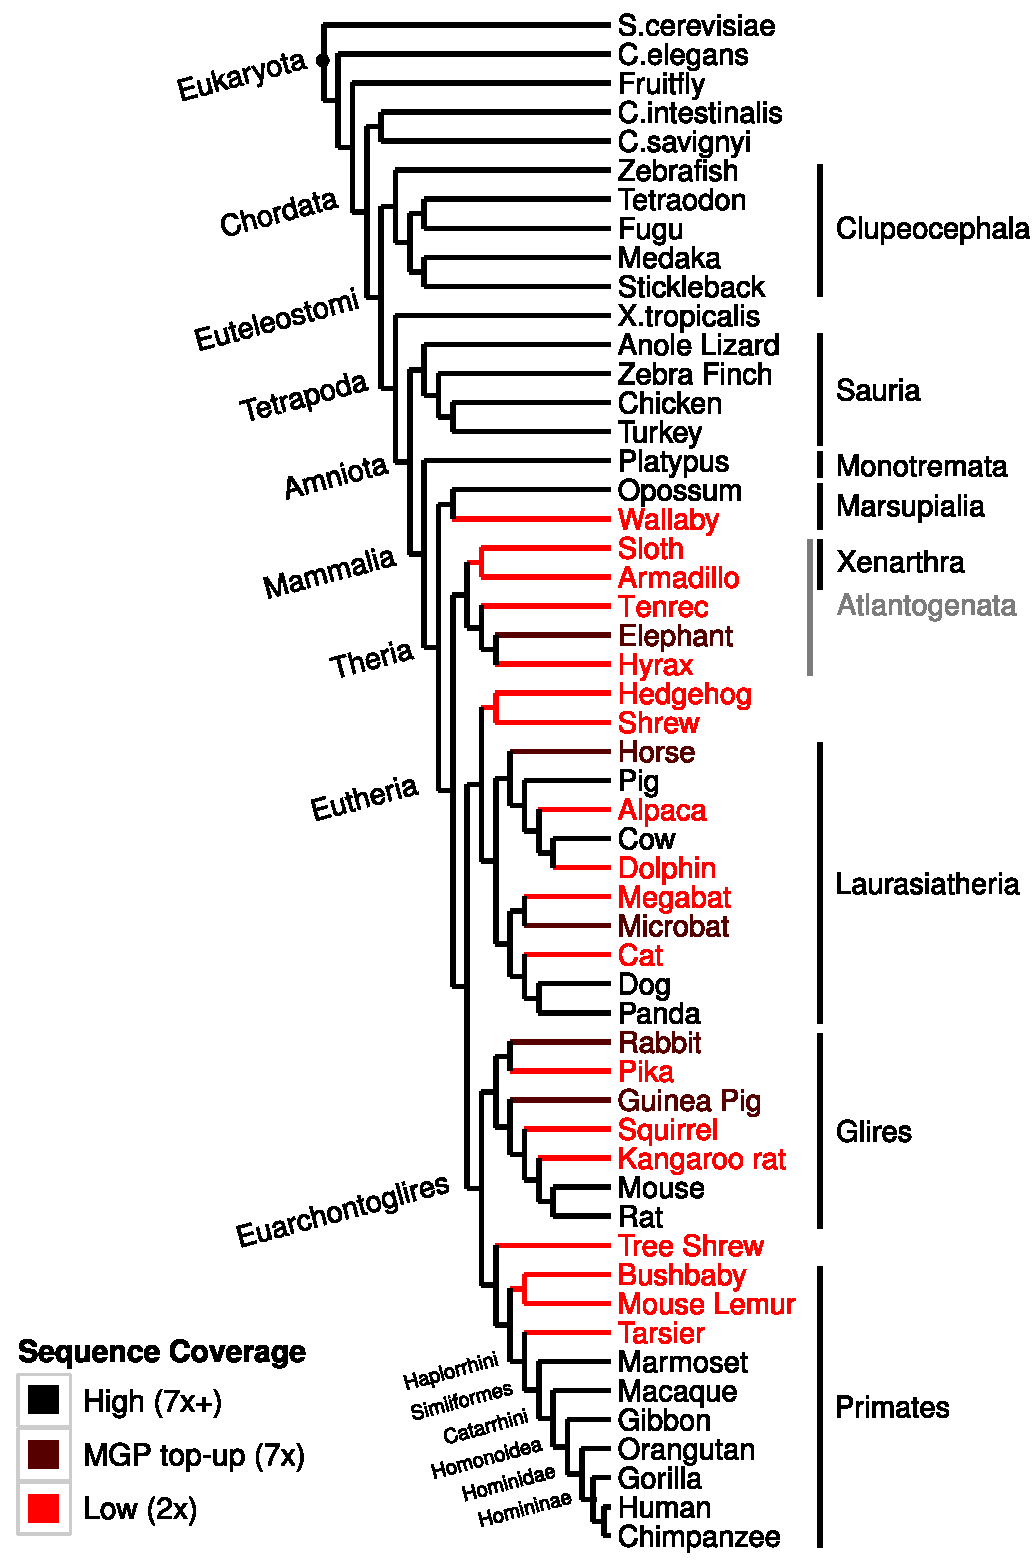
\includegraphics[scale=0.7]{Figs/species_tree.pdf}
\caption{The NCBI taxonomy of species within the Ensembl Compara
  database. Note that branch lengths are not drawn to
  scale. Low-coverage genomes (e.g., those with 2-6x mean sequence
  coverage) are labeled in red, and high-coverage genomes are in
  black. Clade names are included on the left and on the right side of
  the tree.}
\label{ncbi_tree}
\end{figure}


\begin{table} \footnotesize
\centering
\begin{tabular}{@{}lll@{}} \toprule
\multicolumn{2}{c}{Method} \\ \cmidrule(r){1-2}
   Category & Name & Constraints \\ \midrule
Ingroup & Primates & $TC(Primates) > 0.6$ \\
 &   Glires &  $TC(Glires) > 0.6$ \\
 &   Laurasiatheria & $TC(Laurasiatheria) > 0.6$ \\
 &   Sauria & $TC(Sauria) > 0.6$ \\
 &   Fish & $TC(Clupeocephala) > 0.6$ \\
Outgroup &  Eutheria & $TC(Eutheria) > 0.6$ \\
 &   Amniotes & $TC(Amniota) > 0.6$\\
 &   Vertebrates & $TC(Vertebrata) > 0.6$\\
 &   Fungi/Metazoa & $TC(Fungi/Metazoa) > 0.6$\\
Subgroups &  MammalSubgroups & $TC_{all}(Laur., Glires, Primates) > 0.1$\\
 &   \scriptsize{MammalSubgroupsPlusOutgroup} & $TC_{all}(Laur., Glires, Primates) > 0.1$ AND \\
 &    & $TC_{any}(Sauria, Clupeo., Ciona, Marsup.) > 0)$ \\
Orthologs & Human Orthologs & \\
 &   Mouse Orthologs &  \\
 &   Zebrafish Orthologs &  \\
 &   Drosophila Orthologs &  \\
Root Nodes & Ensembl Roots &  \\
\bottomrule
\end{tabular}
\caption{Subtree constraints used for identifying \euth
  orthologous subtrees. Ensembl gene trees were split into subtrees
  based on \acf{tc} requirements at internal
  nodes. Laur. - Laurasiatheria; Clupeo. - Clupeocephala; Marsup. -
  Marsupiala}
\label{subtree_constraints}
\end{table}

The \subtr{} splitting scheme was applied to the 18,607 gene trees
from the \cmp database, producing a set of \subtr{}s for each of the
\acp{tcc} shown in Table \ref{subtree_constraints}. In the next two
sections I will describe the resulting sets of trees and \subtr{}s and
discuss what they reveal about the evolutionary history of vertebrates
and the feasibility of using \acp{tcc} to isolate \mammln \acp{lot} for
sitewise analysis.

\section{Analysis of the set of root Compara gene trees}
\label{section_root_compara_trees}

Table \ref{ensembl_root_table} presents a summary of the set of root
Compara gene trees and the subsets of trees with greater or fewer than
15 sequences.

\begin{table} \footnotesize
\centering
\begin{tabular}{lrb{2cm}rrrrrrr}
\toprule
Tree & &  Med. Size &  & \multicolumn{3}{c}{Human Content} & Human & Med. & Med. \\ \cmidrule(r){5-7}
Set & Count  & (Min / Max) & N50 & 0 & 1 & 2+ & Total & MPL & Species \\ 
  \midrule
\input{Tables/ortholog_roots_summary.txt}
   \bottomrule
\end{tabular}
\caption{Summary of the set of Ensembl Compara root trees. The 'Human
  Content' columns represent the fraction of trees which contain the
  indicated number of human genes, and 'Human Total' is the total
  number of human genes contained within the tree set. 'Med. Species'
  is the median species count across all trees. Med. - median, MPL -
  mean path length }
\label{ensembl_root_table}
\end{table}

A first observation was that, somewhat surprisingly, nearly half of
all \cmp gene trees contained few sequences: 9,378 out of 18,607 root
trees constituted fewer than 15 sequences. Given the protein-based
clustering performed by the Compara pipeline, one might expect many of
these small trees to represent portions of larger fast-evolving gene
trees whose high sequence divergences made the BLAST search step
inaccurate or caused clustering via the \hclust algorithm to be
ineffective. Alternatively, these small gene trees might have resulted
from extensive lineage-specific gene duplications or from pseudogenes
being mis-annotated as genes, in either case causing tight clusters of
very closely-related transcripts that would have been identified by
\hclust as independent clusters of homologs. Some evidence for the
latter scenario could be found in the median species counts and mean
path lengths of the smaller (fewer than 15 sequences) versus larger
(greater than 15 sequences) trees, shown in the second and third rows
of Table \ref{ensembl_root_table}. The set of small root trees had a
median species count of 2, compared to 47 for the large trees,
indicating that the smaller trees encompassed sequences from a very
small taxonomic range. Furthermore, the median \ac{mpl} for small
trees was 0.04 compared to 1.04 for the large subset, revealing a much
smaller level of sequence divergence within each tree. These two
summary statistics together provided evidence that the smallest gene
trees in the \cmp database consist of highly species-specific,
closely-related proteins; it was likely that many of these small trees
represented artifactual gene annotations and would be most
appropriately removed prior to any downstream analysis.

Despite the existence of many small gene trees in the \cmp database,
they comprised only a small fraction of all protein-coding
sequences. Only 809 human genes, or 4\% of the total human gene
set---a gene set which I expected be well-annotated and to contain few
false positive genes due to the high level of manual curation and the
large amount of continued scrutiny---was contained within the subset
of small trees. This indicated that whatever process was causing the
\cmp pipeline to yield a high number of small gene trees did not have
much of an impact on the overall placement of human protein-coding
genes within the database of root \cmp gene trees.

\begin{figure}
\centering
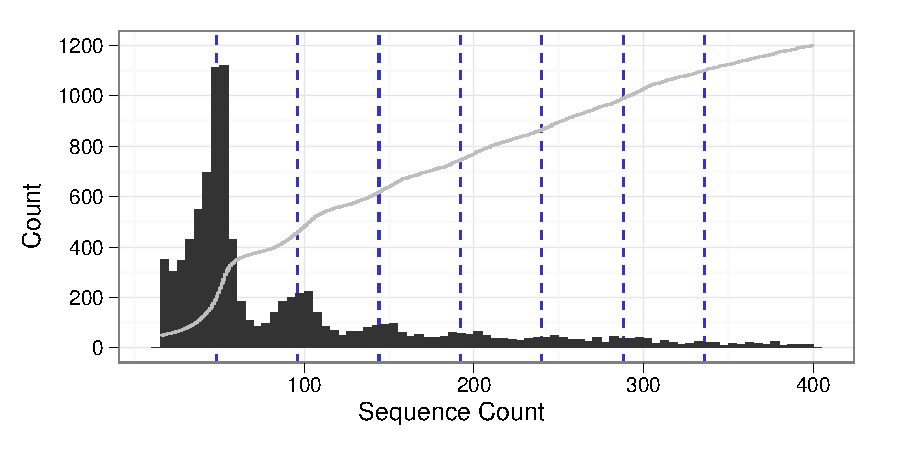
\includegraphics[scale=0.9]{Figs/ensembl_roots_hist.pdf}
\caption{Sequence counts for the set of root Compara trees. Black bars
  show a histogram of sequence counts in bins of width 5, and the gray
  line shows the cumulative fraction of sequences contained within
  trees of that size or smaller. For clarity, 9,378 trees with 15 or
  fewer sequences are not shown. Dashed blue lines are drawn at
  integral multiples of 48, the number of vertebrate species within
  Ensembl.}
\label{ensembl_roots_hist}
\end{figure}

As mentioned in Section \ref{section_quantifying_paralogous}, a closer
examination of the distribution of tree sizes in the set of root \cmp
trees presented a clear view of the over-clustering of \mammln
\acp{lot}. The black bars in Figure \ref{ensembl_roots_hist} show the
distribution of sequence counts for all trees with more than 15
sequences, with vertical dashed lines overlaid at multiples of 48, the
number of vertebrate species in \ens release 63. The highest peak of
the histogram is at or slightly above 48 sequences, with the tree
counts quickly diminishing at larger sizes. Weaker, but still
discernable, peaks exist at larger tree sizes, with the location of
these wave-shaped peaks corresponding closely to the second, third and
fourth multiples of 48. The pattern of recurring peaks is
indistinguishable at sizes above 200, but there is still a long tail
of large trees extending out to a maximum size of 400
sequences. Overall, the distribution of tree sizes provided good
support for the situation described in Section
\ref{section_quantifying_paralogous}, with the \cmp pipeline often
clustering together two or more \mammln \acp{lot} related by a more
distant duplication event.

I found it interesting to characterize the set of root \cmp gene trees
by the proportion of all protein sequences which are covered by trees
of a given size or smaller. This value is plotted in Figure
\ref{ensembl_roots_hist} as a gray line. First, this plot showed that
trees with fewer than 15 sequences (which were excluded from the plot
but inlcuded in the calculation of the cumulative distribution shown)
represented a trifling fraction of the sequences within the \cmp
database; this observation was similar, but not identical, to the
statistic noted above, that only 4\% of human genes were contained
within small trees. Second, the steady upward slope of the cumulative
curve contrasted with the declining height of the histogram bars at
higher sequence counts. This was a result of the increasing number of
sequences encompassed by each of the larger trees: although relatively
few trees contained more than 300 sequences, together they comprised
around 10\% of all protein-coding genes in \cmp. Two points along this
cumulative plot were of particular interest. First, one could use the
height of the cumulative line at the beginning of the second hump in
the histogram (at around 75 sequences) to identify the fraction of
vertebrate proteins which exist in the \cmp database as members of a
duplicated \mammln \ac{lot}. The line showed that around 30\% of
proteins are covered by trees of 75 sequences or fewer, meaning that
70\% of vertebrate proteins are contained within large gene trees
containing sequence-based evidence of ancient paralogy. Second, using
the cumulative line in the reverse direction could identify the tree
size above which 50\% of all sequences were clustered. This value
represents the size of tree that an ``average'' protein might be
clustered in, and in some ways is a more accurate characterization of
a set of gene trees than the median tree size. A similar calculation
is often performed to characterize the size distribution of contiguous
sequence blocks (contigs) within a genome assembly. This statistic,
referred to as the N50 length, is the contig length for which 50\% of
bases are contained in contigs of that size or larger
\citep{Miller2010}. For the \cmp gene trees, the N50 tree size was
139, slightly less than three times the number of vertebrate species
(Table \ref{ensembl_roots_hist}). Thus, the average protein in the set
of \cmp gene trees belonged to a tree with 139 sequences,
corresponding roughly to three \mammln \acp{lot} related by ancient
duplication events, likely resulting from the two rounds of vertebrate
genome duplication.

Another way to characterize the distribution of \cmp gene trees was
across the taxonomic space. Given the wide range of quality in genome
assemblies and annotation sets contained within \ens, a question of
particular interest was whether levels of gene presence and absence
were consistent across different species groups and different levels
of assembly quality. To investigate this question in the context of
the root \cmp gene trees, data were collected by counting the number
of sequences from each species contained within each gene
tree. Results of this analysis are presented in Figure
\ref{ortholog_root_dups}, showing the number of trees containing 0, 1,
2, or more than 3 genes from each of the 53 species within
\ens. Comparing the ranges of values for each copy count (labeled 0,
1, 2 and 3+), I found that the largest number of trees contained zero
copies from any one species (between 8,000--11,000 within vertebrate
species), a smaller but large number of trees contained one copy from
a species (between 4,000-6,000) and several thousand trees contained
two, three or more copies (between 1,000-1,500 for 2 copies and
1,500-2,000 for 3+). Note that these numbers were tabulated
independently between species; for example, the 10,000 \zcop trees in
human were counted independently of the 10,000 \zcop trees in
chimpanzee, so nothing could be said about how many trees contained
zero copies in both human \emph{and} chimpanzee. As noted in the
analysis of tree sizes, the large number of \zcop trees reflected the
large number of small, species-specific trees within the set of \cmp
gene trees. Similarly, the large number of trees with many copies from
each species reflected the trees with multiple \mammln \acp{lot}
clustered together.

Comparing numbers horizontally across the range of species in Figure
\ref{ortholog_root_dups} revealed that the zero-copy count tended to
increase with increased evolutionary distance from human, while the 1,
2 and 3+ copy counts tended to decrease as the distance from human
increased. Both trends were most striking at the distant end of the
tree, where the five non-vertebrate species are shown. For the
increase in \zcop trees and the decrease in single-copy trees, the
strength of the trend at the highest level of divergence can be partly
explained by the long branch lengths connecting those species to each
other and to the more densely sampled vertebrate clade: the
distance-based clustering algorithm might reasonably be expected to
produce more false negatives in longer branches for a number of
reasons, including the behavior of the \hclust algorithm, inaccurate
BLAST E-values at large distances, and heterogeneity in evolutionary
rates across lineages \citep{Whelan2008}. However, the reduced numbers
of 2 and 3+ copy count trees in non-vertebrate species were most
likely due to the whole-genome duplications at the basal vertebrate
lineage, resulting in the non-vertebrate species, which underwent no
such genome duplications, being strongly depleted of multi-copy
duplicates compared to their vertebrate relatives.

Knowing that many of the \lcv genomes were annotated using projections
based on the human set of transcripts, it was slightly concerning that
human and its close primate relatives contained fewer zero-copy genes
and more one-copy and two-copy genes than any other group of
vertebrates in the \cmp set of trees. There was no \emph{ab initio}
biological reason to expect this to be the case, so I suspect that
this pattern, which was fairly small in effect, was due to the
widespread reliance on human annotation and protein experimental data
in the annotation of non-human genomes. There was, however, one region
of Figure \ref{ortholog_root_dups} where human and primates did not
contain the largest number of one-copy or 2-copy trees: the 3+ copy
count for the fish species was greater than that for human or any
primates, which was most likely a result of gene duplicates retained
after the third round of genome duplication in the teleost ancestor
\citep{Jaillon2004}. The signal resulting from the teleost genome
duplication event was clearer in the Fish set of \ac{tc}-defined
\subtr{}s, so I will defer further discussion of this effect to
Section \ref{section_analysis_sets_subtrees} where that set of trees
is described.

Finally, the differences in copy counts between species with low- and
high-coverage genome sequences showed the tendency of \lcv genome
sequences to be absent from gene trees or to show reduced copy
counts. Low-coverage species contain more \zcop, roughly the same
number of one-copy, and noticeably fewer multi-copy genes than
closely-related high-coverage species. These clear differences showed
that gene absence in \lcv genomes should not be taken as evidence for
actual gene loss, and that gene duplications are systematically
underrepresented in \lcv genomes. The former point was emphasized in a
recent critical analysis of the impact of \lcv genomes on gene
duplication inference in the \cmp database \citep{Milinkovitch2010},
but the latter point was largely ignored. Again, this signal was also
stronger in the sets of \ac{tc}-defined \mammln \subtr{}s and will be
revisited in the next section.

The preceding analysis of the set of root \cmp gene trees, in which I
characterized the distribution of trees with respect to size and
across the taxonomic space, showed that despite the
over-representation of small, species-specific trees, most sequences
were contained in trees with biologically plausible sizes given the
history of vertebrate whole-genome duplications. A gene tree-based
equivalent of the N50 statistic was developed for summarizing the
distribution of protein sequences within differently-sized gene trees,
and two visual summaries of this distribution were introduced (in
Figures \ref{ortholog_root_dups} and \ref{ensembl_roots_hist}),
providing evidence for the clustering of paralogous mammalian
sub-trees and for species-based and genome quality-based trends in the
breakdown of gene copy counts within the root \cmp gene trees.

\begin{landscape}
\begin{figure}
\centering
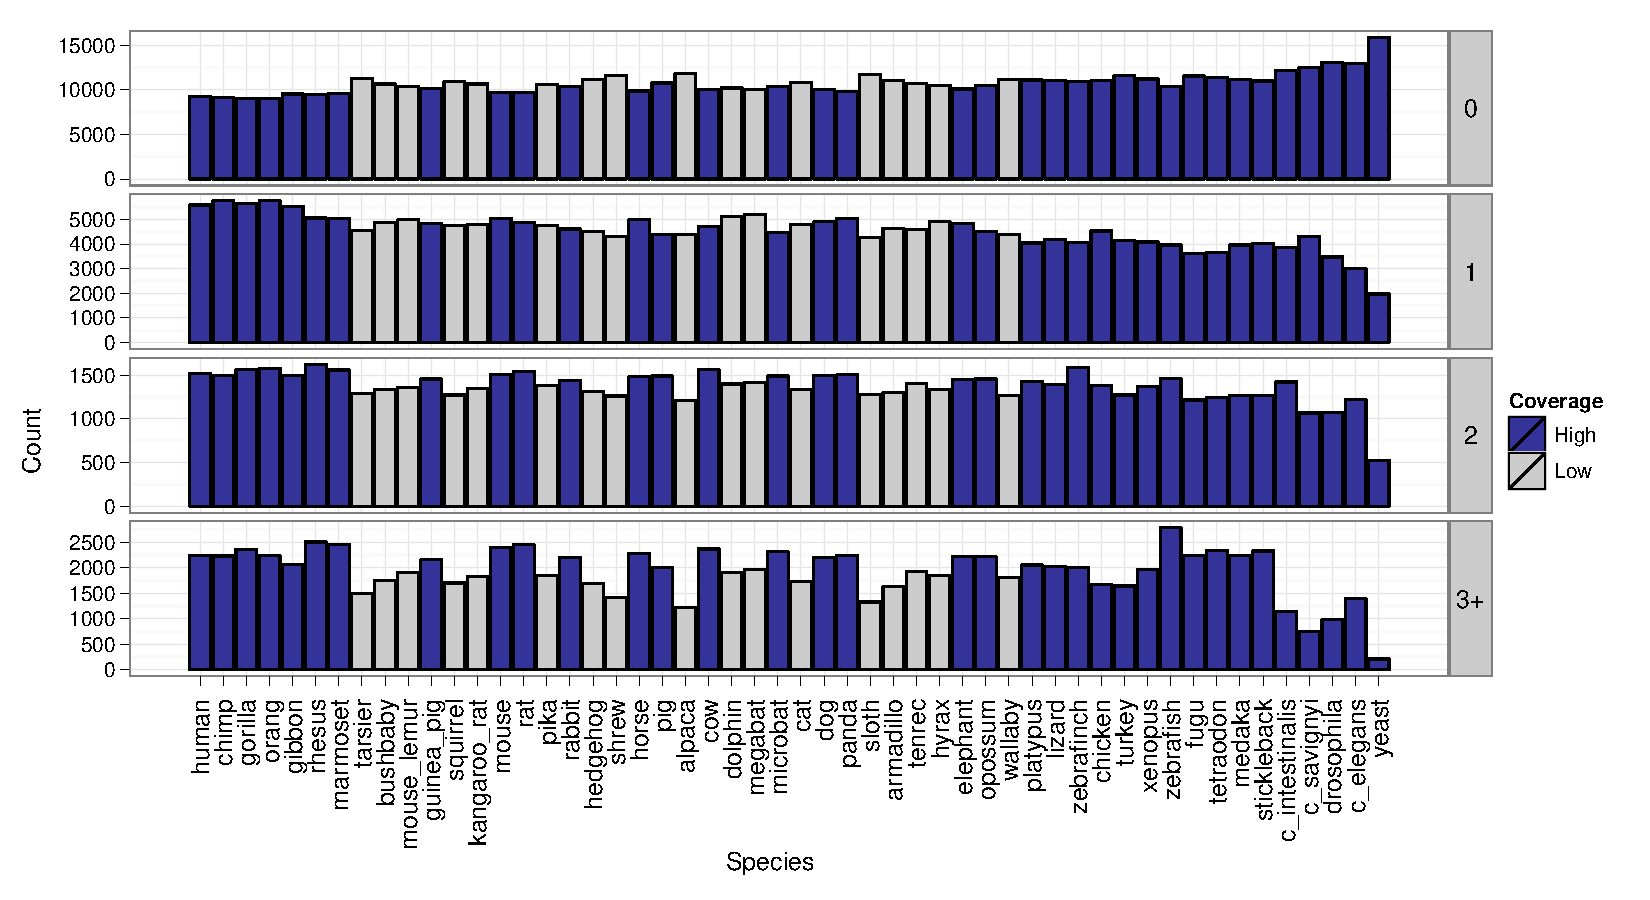
\includegraphics[scale=0.9]{Figs/ortholog_root_dups.pdf}
\caption{Taxonomic distribution of gene copy counts for the root
  Ensembl trees. The number of trees containing 0, 1, 2 or more than 3
  sequences from each species is shown. Bars are colored blue and gray
  for species with high- and low-coverage genomes, respectively. Note
  that the y-axis scale is not the same for each panel.}
\label{ortholog_root_dups}
\end{figure}
\end{landscape}

\section{Analysis of sets of \subtr{}s defined by taxonomic coverage and orthology annotation}
\label{section_analysis_sets_subtrees}

The sets of trees resulting from applying the \subtr splitting scheme
with various \acp{tcc} to the \cmp gene trees are summarised in Table
\ref{ensembl_subtree_table}, with a summary of the root \cmp gene
trees and a summary of the set of seven-species amniote gene trees
from the Optic database \citep{Heger2008} included at the bottom for
comparison.

The Ensembl Roots and Drosophila Orthologs sets were two clear
outliers among the \subtr sets shown in Table
\ref{ensembl_subtree_table}, with much higher N50 values (139 and 125
vs. the next highest value of 56) and more trees with multiple human
copies (0.20 and 0.43 vs. the next highest value of 0.14) than any
other \subtr set. In fact, these two \subtr sets were very similar
except for the excess of small species-limited trees in the Ensembl
Roots set: the Drosophila Orthologs set contained fewer trees than the
Ensembl Roots (9,210 vs. 18,607) and a larger average tree size (60
vs. 15), and the summary values closely resembled the set of Ensembl
Roots with small trees removed (Table \ref{ensembl_root_table}).

Within the Ingroups category, methods based on mammalian \acp{tcc}
(Primates, Glires and Laurasiatheria) produced largely similar sets of
trees, with the Primates set containing around 2,000 more trees and
covering around 1,000 more human genes than the Glires and
Laurasiatheria sets. There was no readily apparent reason for the
higher number and human gene coverage of Primate trees, although it
may speculatively be due to an excess of primate-specific gene trees
that were not captured by non-primate \acp{tcc}. Further investigation
of the trees unique to this set would be required to reveal the root
cause of this minor discrepancy.

The Sauria set of \subtr{}s was noticeably different from the
mammal-based \acp{tcc} sets from the Ingroups category. The Sauria
clade was represented by only four species in Ensembl and diverged
from the \mammln ancestral population at an early point in the
evolution of amniotes; it is plausible that the lower clade size and
long branch length separating Sauria from the other vertebrate clades
caused the moderately lower number of trees (13,046 vs. 15,764 for
Laurasiatheria) and the increased proportion of trees containing
multiple human genes (0.14 vs. 0.09 for Laurasiatheria).

The Fish clade \ac{tcc} produced a strikingly different set of trees,
resulting from the impact of the teleost-specific whole-genome
duplication on the structure of gene trees in fish. Although the Fish
\subtr set yielded a N50 value of 49, which was no different from the
N50 of the other Ingroups sets, Table \ref{ensembl_subtree_table}
highlights three major differences in the Fish set: it contained many
more trees, a higher proportion of trees with zero human copies, and a
lower total human gene count than the other Ingroups sets.

The reason for the drastically different Fish tree set was that the
tree splitting procedure was designed to identify the largest
non-overlapping set of \subtr{}s that satisfied the given
\acp{tcc}. Genes where one or both of the duplicate copies from the
teleost-specific whole-genome duplication were lost would appear as
one-to-one orthologs or deletions with respect to the other vertebrate
lineages. Genes that were retained in duplicate form, however, would
result in a gene tree with two teleost-specific \subtr{}s, each
containing a high \ac{tc} value (i.e., near or equal to 1.0) for the
Clupeocephala clade that contains the fish species within \ens. In
this case, the splitting procedure would produce two small
fish-specific \subtr{}s, ``ignoring'' the surrounding set of mammalain
orthologs because two smaller non-overlapping trees already exceeded
the \ac{tc} threshold of 0.6. If, however, one of the duplicate gene
copies were lost, then the tree would resemble a typical
singly-orthologous vertebrate gene tree, and the splitting procedure
would select a \subtr encompassing the entire vertebrate clade. It
follows that the presence of small, teleost-specific gene trees in the
Fish set is a signal of retained duplicate copies, and the size
distribution of trees from the Fish set, shown in Figure
\ref{ensembl_fish_hist}, shows that several thousand trees fit the
expected model. If we assume that all trees from the Fish subset which
contain zero human copies, span 5 or fewer species, and contain 40 or
fewer sequences are likely retained duplicate genes, a total of 6,980
retained duplicates are identified, yielding a retention rate of
17.5\%, which is very much in line with a previously published
estimate of 15\% based on a comparison of tetraodon, fugu and
zebrafish genes \citep{Brunet2006}.

\begin{figure}
\centering
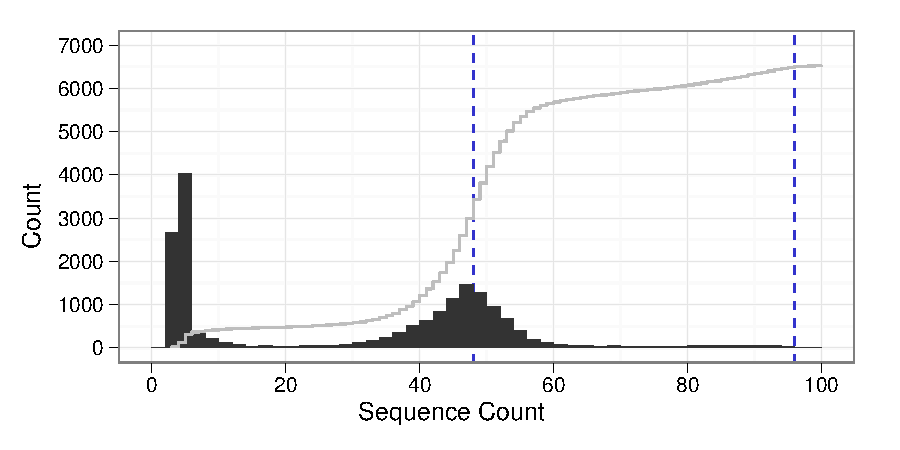
\includegraphics[scale=0.9]{Figs/ensembl_fish_hist.pdf}
\caption{Sequence counts for the set of \subtr{}s identified using the
  Fish clade taxonomic coverage constraint, showing an excess of small
  \subtr{}s resulting from the teleost genome duplication. Black bars
  show a histogram of sequence counts in bins of width 2, a gray line
  shows the cumulative fraction of sequences contained within trees of
  that size or smaller, and dashed blue lines are drawn at integral
  multiples of 48, the number of vertebrate species within
  Ensembl. Trees with more than 100 sequences are included in the
  topmost bin.}
\label{ensembl_fish_hist}
\end{figure}

The sets of \subtr{}s resulting from the Outgroup methods were of
special interest, as the clades used to define these \acp{tcc}
contained all or nearly all of the \mammln species whose orthologous
genes I wished to study. The resulting sets of \subtr{}s showed little
variation, owing perhaps to the large sizes of the clades and their
similar species composition. Each \subtr set contained between 15 to
17 thousand trees, N50 values of around 49, and greater than 90\% of
trees containing exactly one human sequence. These measures provided
strong evidence that the tree-splitting method was accurately
isolating \mammln \acp{lot}.  Some slight differences between \subtr
sets were apparent, however, with the tree count decreasing, the
proportion of trees with human duplications increasing, and the
overall human gene coverage decreasing as the clade size used for the
\ac{tc} calculation increased. These trends could potentially be
explained by the minimum required tree size increasing along with the
clade size, as a result of the increased number of species required to
produce a \ac{tc} value of 0.6. The minimum \subtr size ranged from 21
for Eutheria to 32 for Fungi/Metazoa.

The Subgroups methods did not appear to produce \subtr{}s of any
higher quality or more biological interest than the Outgroups
methods. The MammalsSubgroups set produced more trees than the
Outgoups sets, but the N50 was slightly lower (46 vs. 49) and the
proportion of \zcop human trees was higher (0.18 vs. 0.01), suggesting
that the additional trees in the MammalsSubgroups set were spurious
\subtr{}s containing limited species coverage. The addition of an
outgroup requirement to the MammalSubgroupsPlusOutgroup method
produced a tree set more closely resembling the Outgroup methods, but
the human gene coverage was lower than that for any Outgroup method
despite the overall higher tree count.

Finally, the ortholog annotation-derived \subtr{}s provided for an
interesting comparison between the three different ortholog sources
and between the overlapping and non-overlapping sets of \subtr{}s. The
\species{Drosophila} ortholog set was highly contrasted with the
vertebrate sets due to the two rounds of whole genome duplication,
while there was minimal variation among the other ortholog sets. It is
interesting to note that the protein-coding transcripts used by the
\cmp pipeline included 21,873 mouse protein-coding genes and only
19,991 human genes, indicating either a larger number of true
protein-coding genes in mouse or a higher tolerance for false positive
gene predictions in the mouse genome compared to the human
genome. Zebrafish, on the other hand, contained 24,540 genes; this
number agreed well with the 17.5\% proportion of retained duplicate
genes that I estimated earlier in this section. Overall, 76\% and 81\%
of mouse and zebrafish genes contained an apparent orthologous
relationship with one human gene, which was only slightly lower than
the 92\% of Eutheria \subtr{}s containing one human sequence.

\begin{landscape}
% latex table generated in R 2.13.0 by xtable 1.5-6 package
% Thu Sep 15 11:19:59 2011
\begin{table}
\centering
\begin{tabular}{llrb{2.5cm}rrrrrrr}
\toprule
\multicolumn{2}{c}{Subtree Method} & &  Med. Size &  & \multicolumn{3}{c}{Human Content} & Human & Med. & Med. \\ \cmidrule(r){6-8} \cmidrule(r){1-2}
Category & Name & Count  & (Min / Max) & N50 & 0 & 1 & 2+ & Total & MPL & Species \\ 
  \midrule
\input{Tables/ortholog_summary.txt}
\bottomrule
\end{tabular}
\caption{Summary of Ensembl \subtr{}s identified using taxonomic
  criteria or Ensembl ortholog annotations. The set of \cmp gene trees
  from Table \ref{ensembl_root_table} and the set of trees from the
  Optic database \citep{Heger2008} are included at the bottom for
  comparison. Cells in numeric columns are shaded according to their
  value relative to other rows, with low values in white and high
  values in blue. The 'Human Content' columns represent the fraction
  of trees which contain the indicated number of human
  genes. 'Med. Species' is the median species count across all
  trees. Med. -- median, MPL -- mean path length}
\label{ensembl_subtree_table}
\end{table}
\end{landscape}

In order to easily compare patterns between \subtr sets and across the
taxnomic space, I tabulated gene copy counts within each \ens species
for each generated \subtr set; the results of this analysis are shown
in Figure \ref{ortholog_stacked_bar}. By way of reference, the values
shown in each of the separate panels of Figure
\ref{ortholog_root_dups} appear in the bottom panel of Figure
\ref{ortholog_stacked_bar} as stacked bars of different
colors. Although the various summary characteristics of each of the
\subtr methods have already been discussed at length, this more
taxonomic-oriented view revealed some salient features of the patterns
of gene deletion and duplication within the tree sets and showed the
pervasive impact of genome-wide duplications on the evolution of
vertebrate genes. The large fraction of species with multiple copies
in the Drosophila Orthologs \subtr set (Figure
\ref{ortholog_stacked_bar}, blue and purple bars) showed the effect of
two rounds of vertebrate genome evolution, producing a large number of
trees with multiple Drosophila orthologs in vertebrate species;
similarly, the elevated fraction of multi-copy fish trees in the
Outgroups \subtr sets (e.g., the blue bars in the Eutheria panel of
Figure \ref{ortholog_stacked_bar}) showed the impact of the
teleost-specific duplication event on the number of \mammln{}
\acp{lot} with multiple fish copies.

\begin{figure}
\centering
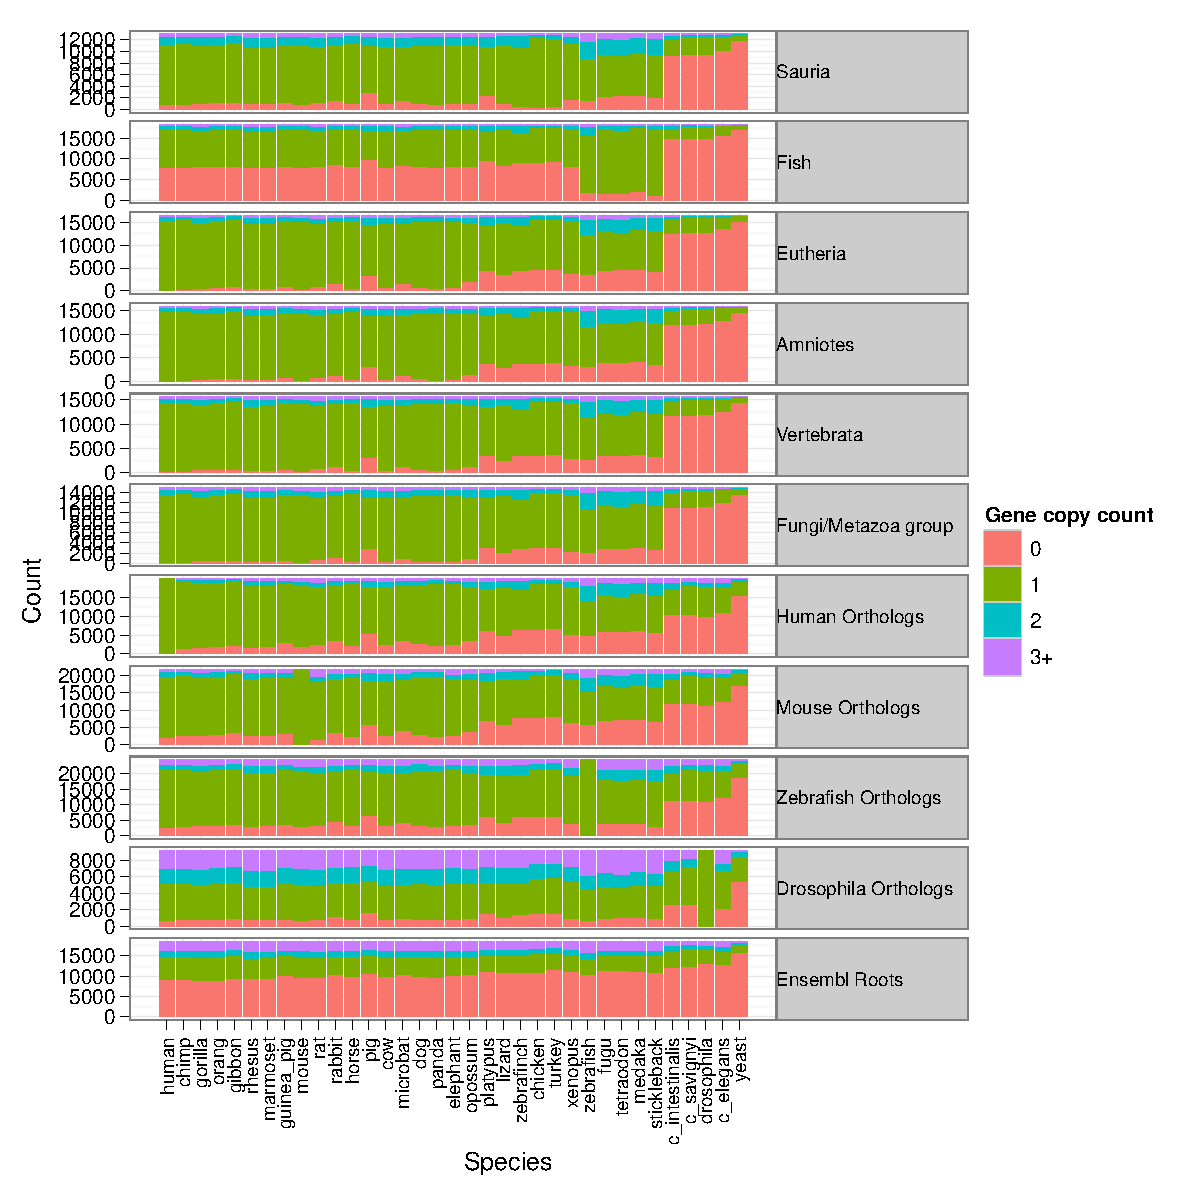
\includegraphics[scale=0.8]{Figs/ortholog_stacked_bar.pdf}
\caption{Taxonomic distribution of gene copy counts for different
  \subtr methods. The numbers of trees containing 0 (red), 1 (green),
  2 (blue) or more than 3 (purple) sequences from each species are
  shown as stacked colored bars. The Ingroup and Subgroups methods
  were omitted for clarity, as were species with low-coverage
  genomes. Note that the y-axis scale is not the same for each panel.}
\label{ortholog_stacked_bar}
\end{figure}

\section{Gene duplication and loss in the set of Eutherian largely orthologous trees}

The \subtr{}s defined by the Eutheria \ac{tcc} were chosen as the
final set of gene trees for use in the downstream sitewise
analysis. This set was chosen due to its slightly larger number of
trees and better coverage of human genes compared to the other \subtr
sets from the Outgroups category (Table \ref{ensembl_subtree_table}).

The distribution of tree sizes for the set of Eutherian \subtr{}s is
shown in Figure \ref{ensembl_euth_hist}. The histogram of tree sizes
showed a single peak at exactly the number of vertebrate species in
\ens, with no trees containing fewer than 20 sequences and a few
hundred trees with more than 100 sequences. The distribution of tree
sizes was consistent with the set of 16,477 gene trees representing an
accurate set of genome-wide \mammln \acp{lot}, with variations in
sequence counts resulting from sporadic gene duplication or loss
events or unannotated genes in \lcv genomes.

\begin{landscape}
\begin{figure}
\centering
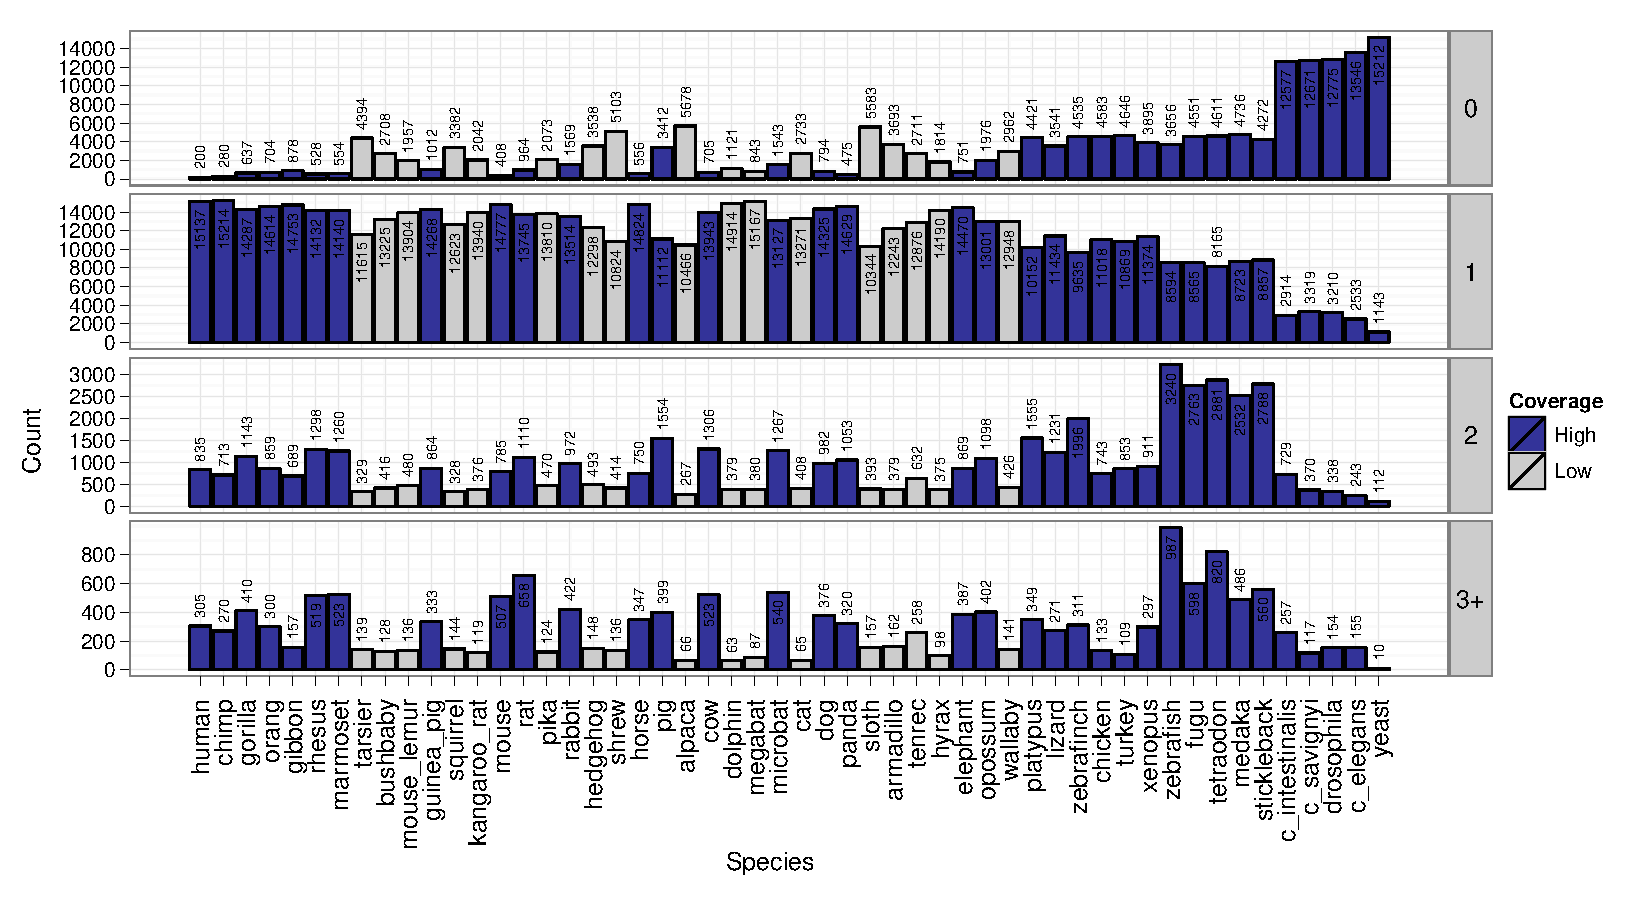
\includegraphics[scale=0.9]{Figs/ortholog_euth_dups.pdf}
\caption{Taxonomic distribution of gene copy counts for the Eutheria
  \subtr{}s defined by taxonomic coverage constraints. Each panel from
  top to bottom shows the number of trees containing 0, 1, 2 or more
  than 3 sequences from each species. Bars are colored blue and gray
  for species with high- and low-coverage genomes, respectively. Note
  that the y-axis scale is not the same for each panel.}
\label{fig_ortholog_euth_dups}
\end{figure}
\end{landscape}

I also analyzed the detailed taxonomic distribution of gene
duplications and losses implied by the set of Eutherian \subtr{}s, as
the relative prevalence of zero-copy and multi-copy trees in this set
of \acp{lot} might provide some indication of whether gene deletion or
gene duplication has been more prevalent in the evolution of
vertebrate genomes. Figure \ref{fig_ortholog_euth_dups} shows the gene copy
counts for the set of Eutherian \subtr{}s across all \ens species,
similar to what Figure \ref{ortholog_root_dups} showed for the set of
root \cmp gene trees. The excess of \zcop trees and deficit of
duplications in \lcv genomes was immediately apparent from Figure
\ref{fig_ortholog_euth_dups}, confirming the trend observed in the set of
root \cmp trees. Similarly, the trend of increased \zcop trees in
non-mammalian and non-vertebrate species was stronger than in Figure
\ref{ortholog_root_dups}, as was the excess of trees with multiple
copies in fish genomes.

A quantitative comparison of the number of multi-copy versus zero-copy
trees in each species showed that gene duplication has had a greater
apparent impact on gene copy counts than gene deletion, at least
within primates and most mammals with high-coverage genomes. For
example, human contained 200 zero-copy trees and 1,140 combined two-
or three-copy trees within the set of Eutherian \subtr{}s, showing
evidence for a greater prevalence of gene duplication than gene
deletion in \acp{lot} since the common Eutherian ancestor. On the
other end of the spectrum in primates was gibbon, which had the most
\zcop trees (878) and the fewest multi-copy trees (846) of all the
primates, showing roughly equal tendencies towards gene deletion and
duplication across the set of Eutherian \acp{lot}. This pattern was
consistent across the mammalian tree, save for a few exceptions:n
guinea pig showed roughly the same number of zero-copy and multi-copy
trees (1012 vs. 1197, respectively), rabbit showed slightly more
zero-copy trees (1569 vs. 1394), and pig showed a much higher number
of zero-copy trees (3412 vs. 1953). Beginning with opossum,
vertebrates more distantly related to the Eutherian common ancestor
showed greater numbers of \zcop trees, leveling off at ca. 4,000
zero-copy trees, and higher variation in the number of multi-copy
genes; at the low end were chicken and turkey with 876 and 972
multi-copy genes, respectively, and at the high end (excluding the
fish species) were zebrafinch and platypus with 1904 and 2307
multi-copy genes, respectively.

In the analysis of vertebrate genomes, one must be vigilantly aware of
potential biases arising from the frequent reliance on homology with
the well-annotated human and mouse genomes in the annotation of newly
sequenced genomes. Such a bias could have plausibly led to anomalous
results in the present analysis of gene copy counts, for example by
reducing the chance of correctly identifying gene trees containing
deletions in human or mouse, thus over-inflating the prevalence of
duplications versus deletions. The level of consistency seen in the
relative numbers of \zcop and multi-copy trees across the range of
mammals provided some evidence against such a bias, although it did
not entirely rule out the possibility, as all mammalian genomes may
have been similarly affected by the use of human or mouse proteins in
the \ens gene annotation pipeline.

An unexpected result of the compraison between mammalian species was
the identification of certain genomes with uncharacteristically high
numbers of \zcop or multi-copy trees. The most striking example was
pig, which contained nearly double the number of \zcop trees of any
other high-coverage \mammln genome and a noticeably elevated number of
multi-copy trees, but rabbit and guinea pig also deviated from the
normal patterns. Given the otherwise consistently low number of \zcop
trees throughout the range of Eutherian mammals, I would expect the
number of \zcop trees in these species to decrease as finished-quality
genome sequences ad produced and the gene annotation pipelines are
further optimized to work with each species. In particular the
anomalous nature of the pig gene trees may be related to the draft
quality of the genome sequence and assembly; I would expect the number
of \zcop trees to be substantially reduced once a finished-quality
genome sequence and annotation set is made available
\citep{Archibald2010}.


\section{Comparison to gene trees from the Optic database of amniote orthologs}

\begin{figure}[t!]
\centering
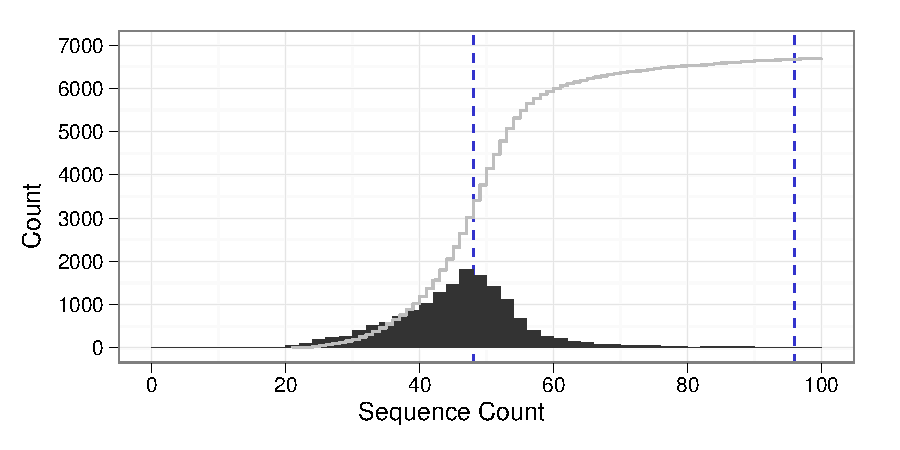
\includegraphics[scale=0.8]{Figs/ensembl_euth_hist.pdf}
\caption{Sequence counts for the set of \subtr{}s identified using the
  Eutheria clade taxonomic coverage constraint. Black bars show a
  histogram of sequence counts in bins of width 2, a gray line shows
  the cumulative fraction of sequences contained within trees of that
  size or smaller, and dashed blue lines are drawn at integral
  multiples of 48, the number of vertebrate species within
  Ensembl. Trees with more than 100 sequences are included in the
  topmost bin.}
\label{ensembl_euth_hist}

\hspace{.2in}

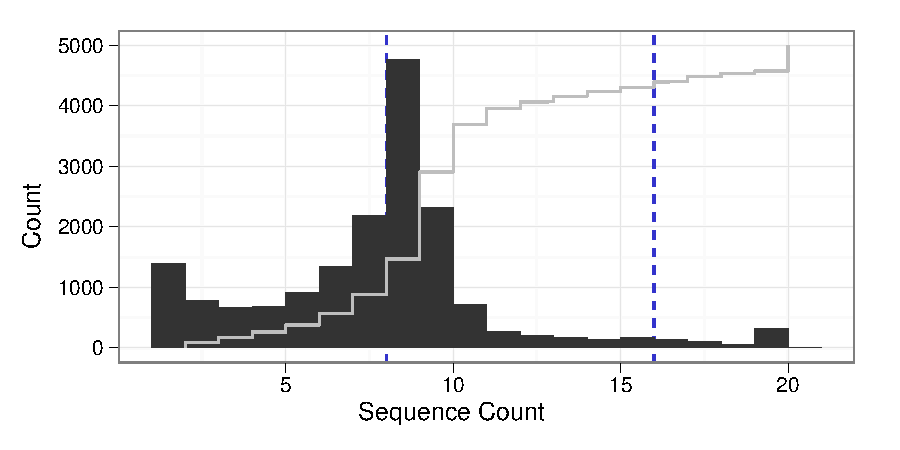
\includegraphics[scale=0.8]{Figs/optic_roots_hist.pdf}
\caption{Sequence counts for gene trees in eight amniote species from
  the Optic orthology database \citep{Heger2008}. Black bars show a
  histogram of sequence counts, a gray line shows the cumulative
  fraction of sequences contained within trees of that size or
  smaller, and dashed blue lines are drawn at integral multiples of 8,
  the number of amniote species analyzed by Optic. Trees with more
  than 20 sequences are included in the topmost bin.}
\label{optic_roots_hist}
\end{figure}

Given the tendency of the root \cmp gene trees to contain multiple
\mammln \acp{lot}, I wished to evalute whether a different
phylogenetic tree-based orthology pipeline produced a similar
distribution of gene tree sizes. The Optic database, a project from
the Ponting group which used an independently designed gene-building
and comparative genomics pipeline combined with the TreeBeST software
to infer duplication-resolved gene trees within a variety of
vertebrate and invertebrate clades, was ideal for such a comparison
\citep{Heger2008}. I downloaded the set of Optic gene trees inferred
from a group of eight vertebrate genomes (human, mouse, dog, opossum,
platypus, chicken, zebrafinch, and tetraodon), characterized the set
of gene trees using a variety of summary statistics, which are
included in the bottom row of Table \ref{ensembl_subtree_table}, and
plotted the distribution of gene tree sizes in Figure
\ref{optic_roots_hist}.

After accounting for differences in the number of sampled species, the
set of Optic gene trees more closely resembled the set of Eutherian
\subtr{}s than the root \cmp gene trees. Nearly 80\% of the Optic
gene trees contained exactly one human sequence and only 9\% contained
two or more human sequences; the large proportion of single-copy trees
suggested that the Optic trees did not contain many ``over-clustered''
\mammln \acp{lot}, and the 9\% of trees with multiple human genes was
close to the 7\% seen in the set of Eutherian \subtr{}s. Figures
\ref{ensembl_euth_hist} and \ref{optic_roots_hist} clearly show the
similar sequence count distributions between the Optic and Eutherian
trees; each histogram has a distinct peak at a sequence count
corresponding to the number of species included in the database, with
no sign of the long tail of large gene trees seen for the distribution
of root \cmp gene trees in Figure \ref{ensembl_roots_hist}.

\section{Conclusions}

This chapter was concerned with identifying a set of gene trees for
subsequent sitewise evolutionary analysis. Three characteristics were
desired in the ideal set of trees: maximal coverage of available
mammalian genomes, minimal inclusion of paralogous relationships, and
consistent taxonomic representation throughout the set of trees. I
chose the \ens \cmp database as a source of root gene trees due to its
well-established methodology \citep{Heger2008,Vilella2009} and its
increased species sampling compared to equivalent vertebrate databases
such as Treefam and Optic.

Using the set of root \cmp gene trees as a basis for further analysis,
I characterized the distribution of gene trees in a varity of ways,
including a tree-based analogue of the N50 statistic commonly used in
evaluating genome assemblies. This analysis showed that the
``over-clustering'' of multiple Eutherian \acp{lot} within single \cmp
gene trees had a major impact on the composition of the gene tree
set. I then developed a simple scheme for isolating \acp{lot} from
within larger gene trees using flexible \acp{tcc} and applied the
system to the set of \cmp trees to generate several sets of
genome-wide \ac{tc}-defined \subtr{}s.

These sets of \ac{tc}-defined \subtr{}s provided a number of insights
into the orthology and paralogy relationships within and between
mammalian and vertebrate genomes, including a quantification of the
proportion of duplicate genes that were retained after the teleost
whole-genome duplication that matched the prediction resulting from a
detailed analysis of fish genomes \citep{Brunet2006}. The comparison
between \subtr{} sets resulting from different \acp{tcc} showed that a
simple threshold based on \ac{tc} in the Eutheria clade produced a set
of \subtr{}s that contained a high percentage of human genes and
satisfied the three desired characteristics for subsequent sitewise
analysis.

An analysis of the number of trees with zero, one, two or more
sequences for a given species revealed patterns of variation in gene
copy counts across vertebrate genomes. Importantly, \lcv genomes
showed a large increase in zero-copy trees (e.g. trees with no
sequences from the low-coverage genome) and a notable decrease in
multi-copy trees. Other, more subtle trends were identified, including
individual genomes, such as pig, with apparently anomalous numbers of
zero- or multi-copy trees, and more widespread trends, such as the
relatively few multi-copy trees in avian genomes and the higher
prevalence of multi-copy trees versus zero-copy trees within mammals.

The set of Eutherian \acp{lot} identified in this chapter represented,
to my knowledge, the largest and most accurate set of mammalian
orthologous trees identified to date. Although the set of Eutherian
\subtr{}s were isolated from the \cmp root trees and not independently
derived, the separation of the ``over-clustered'' \cmp trees into
biologically realistic sets of Eutherian genes sharing mostly
orthologous relationships was an important and fundamental part of
preparing these gene trees for subsequent evolutionary
analysis.

One might argue that a gene tree with fully-resolved duplication and
speciation events, as provided by the \cmp database, should be enough
to allow for identification of orthologous versus paralogous
\subtr{}s. In theory this is true, but such an approach to identifying
\acp{lot} would have failed on two grounds: first, it would not
distinguish between ancient paralogs resulting from the two rounds of
whole-genome duplication in vertebrates and more recent paralogs
resulting from the gradual accrual of gene duplications over time,
causing recent duplication events to be handled in the same way as
ancient duplications absent the incorporation of taxonomic
information. Second, in practice the resolution of gene deletions
within the \cmp gene trees was far from perfect, a point raised by
Milinkovitch et al. \citeyearpar{Milinkovitch2010} in their criticism
of the inclusion of \lcv genomes in the \ens \cmp orthology
pipeline. A lack of data, caused either by missing genes from \lcv
genomes or by the limited amount of sequence data available for
phylogenetic reconstruction, may often contribute to errors in the
accurate identification of duplication and speciation nodes within the
\cmp gene trees; the use of \ac{tc} information sidestepped this
source of uncertainty by not relying on accurate resolution of
duplication nodes.

The performance of the \ac{tc}-based scheme described in this chapter
showed that simple taxonomic criteria could be used to identify
largely orthologous subtrees. The utility of a taxonomic-based
approach to identifying meaningful gene tree \subtr{}s was indirectly
validated by comparison to gene trees from the Optic orthology
database, which showed many similar characteristics to the set of
Eutherian \subtr{}s; the pipeline used to create the Optic database
includes an explicit step for splitting trees based on taxonomic
criteria \citep{Heger2008}, suggesting that a similar technique was
found to be important in identifying \acp{lot} within the context of
an independently designed orthology pipeline.
